\section{Kontroles iekārtas pilnais kods} \label{appx:control}
\lstinputlisting[language={[qucs]VHDL},%
                caption={Kontroles iekārtas VHDL apraksts. (\texttt{control2.vhd})},%
                label=kb:control,
                emph={state,branchTest},%
                breaklines,breakatwhitespace,
                basicstyle=\ttfamily\scriptsize ]{code/control2.vhd}

\clearpage
\section{Atmiņas dekodera pilnais kods} \label{appx:mmu}
\lstinputlisting[language={[qucs]VHDL},%
                caption={Atmiņas dekodera VHDL apraksts. (\texttt{mmu.vhd})},%
                label=kb:mmu,
                %emph={state,branchTest},%
                breaklines,breakatwhitespace,
                basicstyle=\ttfamily\scriptsize ]{code/mmu.vhd}

%\clearpage
%\section{RAM pilnais kods} \label{appx:ram-code}
%\lstinputlisting[language={[qucs]VHDL},%
                %caption={RAM VHDL apraksts. (\texttt{mem.twoport.vhd})},%
                %label=kb:ram,
                %%emph={state,branchTest},%
                %breaklines,breakatwhitespace,
                %basicstyle=\ttfamily\scriptsize ]{code/mem.twoport.vhd}

\clearpage
\section{Simulācijas rezultāti (rev.~02)} \label{appx:simulation}
% MEMORY DUMP "language" definition
\lstdefinelanguage{memdump}
{
	keywordsprefix=@,
	comment=[l]{//}
}

\lstinputlisting[language={memdump},
                 caption={Atmiņas saturs pirms programmas izpildes.},
                 label=kb:mem-before,
                 basicstyle=\ttfamily\small,
                 firstline=4,firstnumber=4]{code/gen/before8.mem}

\lstinputlisting[language={memdump},
                 caption={Atmiņas saturs pēc programmas izpildes.},
                 label=kb:mem-after,
                 basicstyle=\ttfamily\small,
                 firstline=4,firstnumber=4]{code/gen/after8.mem}

\lstinputlisting[language={},
                 caption={Atmiņas satura izmaiņas.},
                 label=kb:mem-diff,
                 basicstyle=\ttfamily\small,]{code/gen/mem8.diff}

\begin{sidewaysfigure}
	\centering
	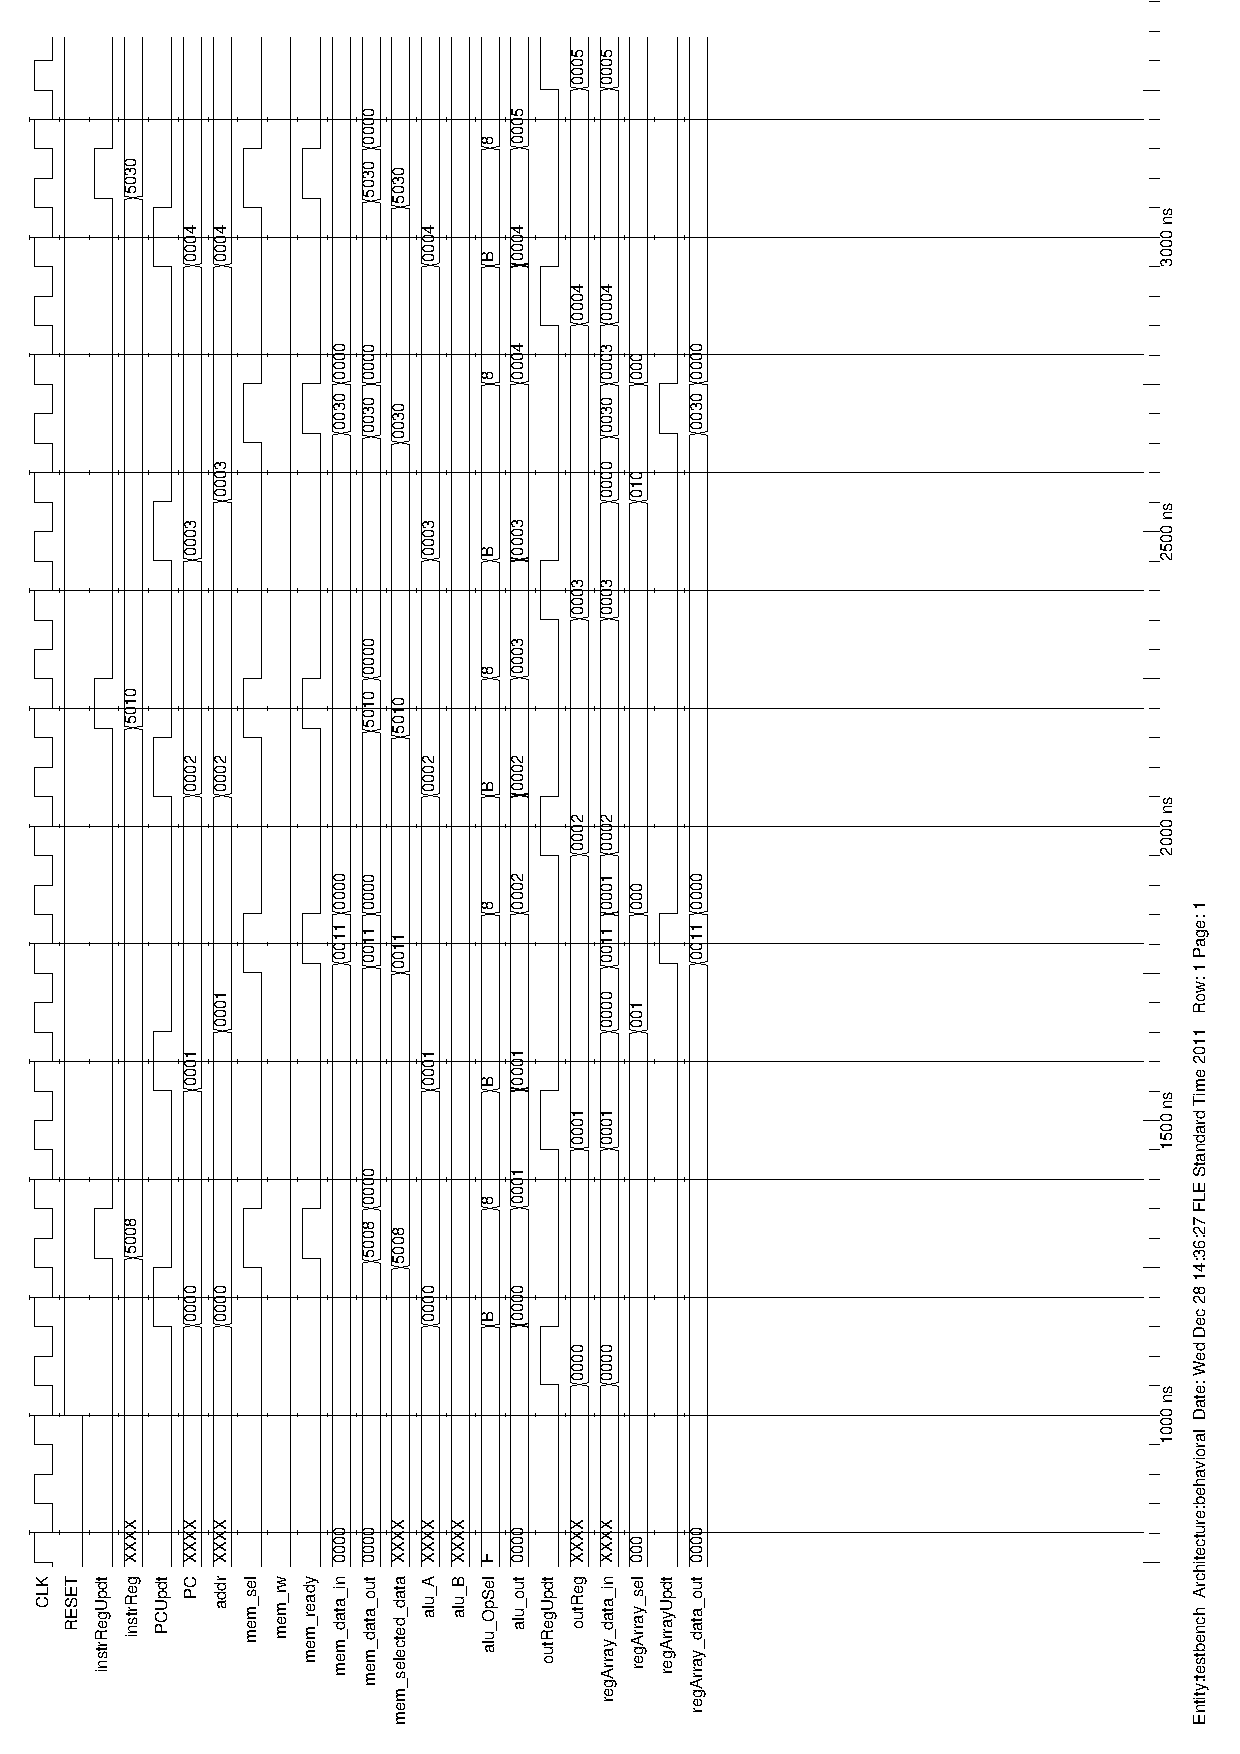
\includegraphics[trim = 0cm 0cm 8cm 0cm,clip,angle=-90,width=\linewidth]{sim0-init}\\
	\caption{Inicializācijas laika diagramma.}
	\label{fig:sim-init}
\end{sidewaysfigure}

\begin{sidewaysfigure}
	\centering
	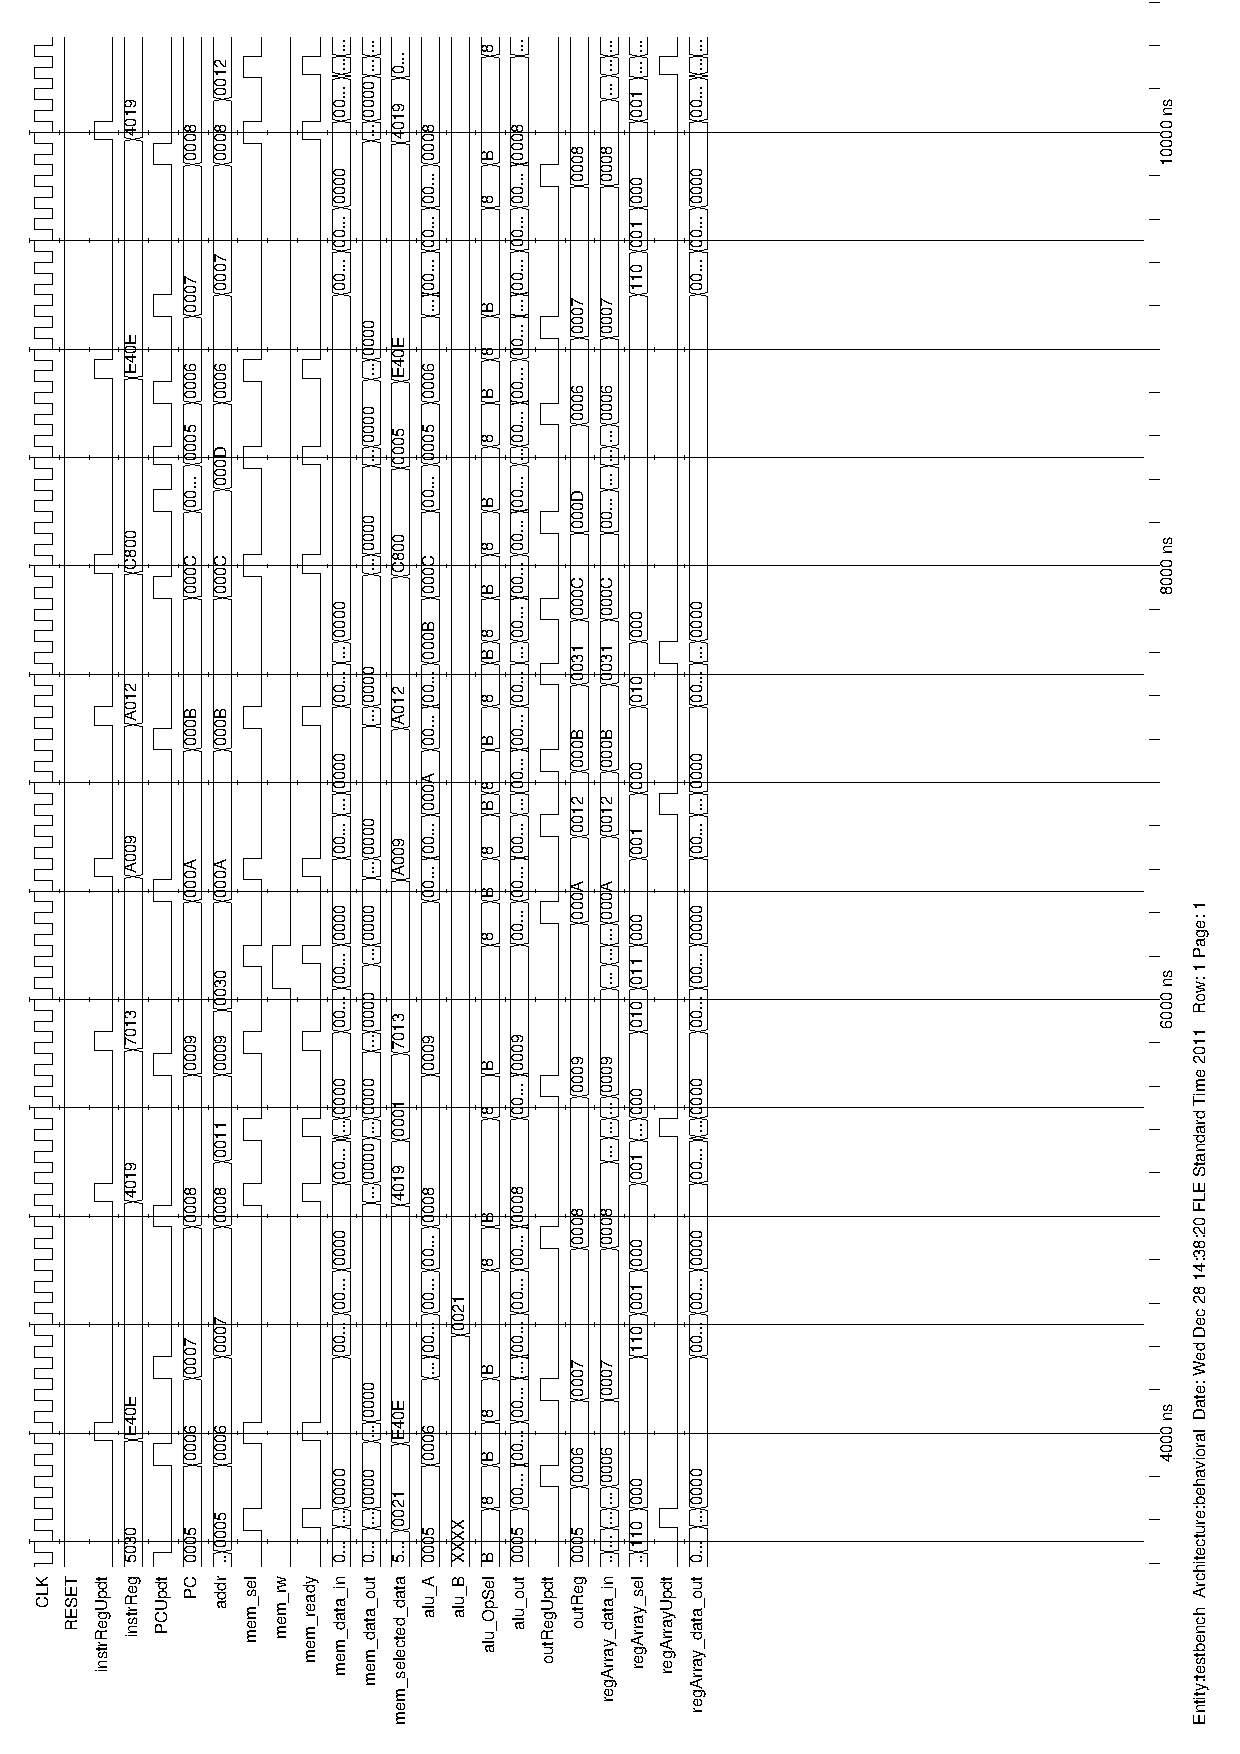
\includegraphics[trim = 0cm 0cm 8cm 0cm,clip,angle=-90,width=\linewidth]{sim0-cycle}\\
	\caption{Programmas cikla izpildes laika diagramma.}
	\label{fig:sim-cycle}
\end{sidewaysfigure}

\begin{sidewaysfigure}
	\centering
	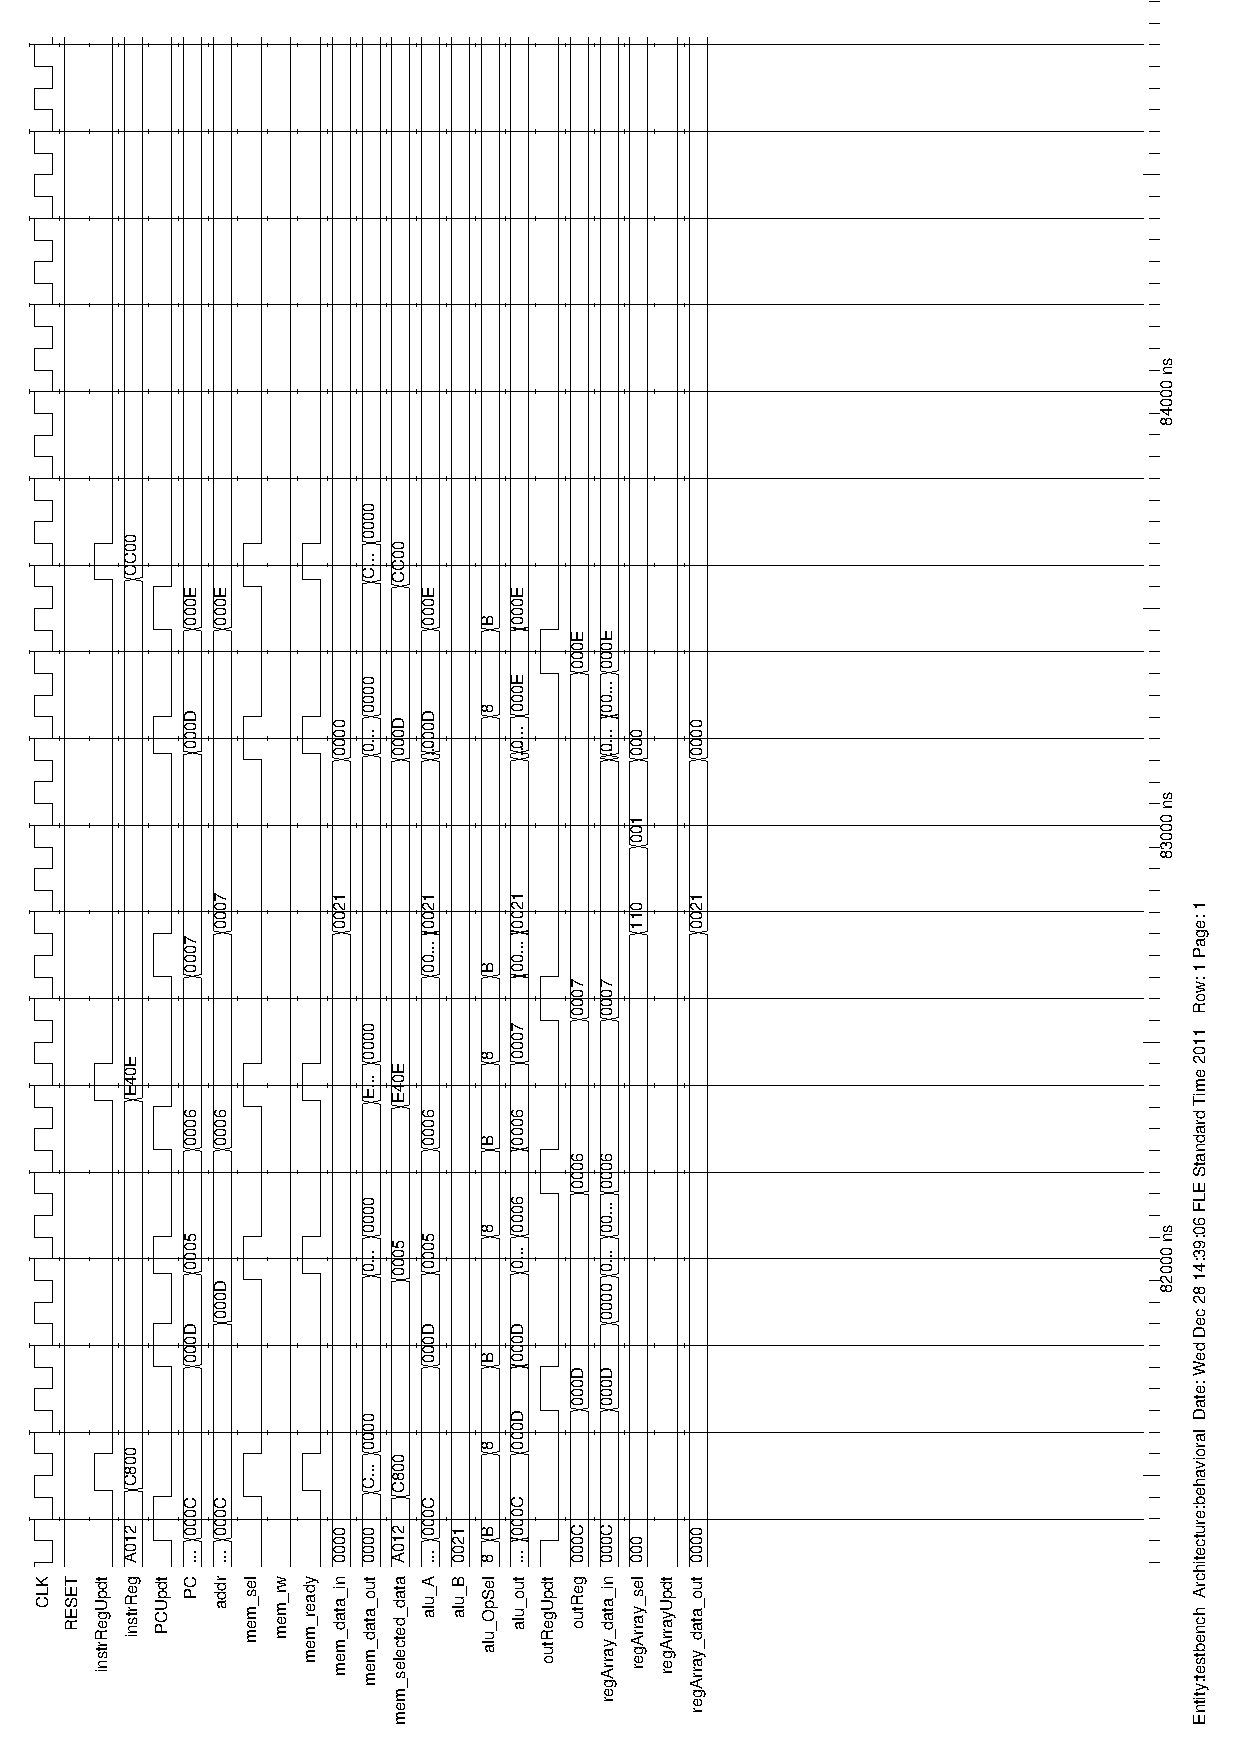
\includegraphics[trim = 0cm 0cm 8cm 0cm,clip,angle=-90,width=\linewidth]{sim0-halt}\\
	\caption{Programmas izpildes beigu laika diagramma.}
	\label{fig:sim-halt}
\end{sidewaysfigure}

\lstinputlisting[float=p,
                 language={JSI},
                 caption={Testa programmas asemblerkods.},
                 basicstyle=\ttfamily\scriptsize,
                 label=kb:copy-program]{code/gen/copy-noaccents.asm}

\clearpage
\section{Paraugimplementācijas asemblerkoda galvene (rev.~03)}
\lstinputlisting[%float=hp,
                 language={JSI},
                 caption={Galvene asemblera programmām (\texttt{JISonFUSIONr3.inc}).},
                 basicstyle=\ttfamily\scriptsize,
                 label=kb:asm-header]{code/JSIonFUSIONr3.inc}

\clearpage
\section{Sāknēšanas programma un simulācijas rezultāti (rev.~03)} \label{appx:boot}
\lstinputlisting[%float=hp,
                 language={JSI},
                 caption={Sāknēšanas programmas asemblerkods.},
                 basicstyle=\ttfamily\scriptsize,
                 label=kb:boot]{code/boot.asm}

\begin{sidewaysfigure}
	\centering
	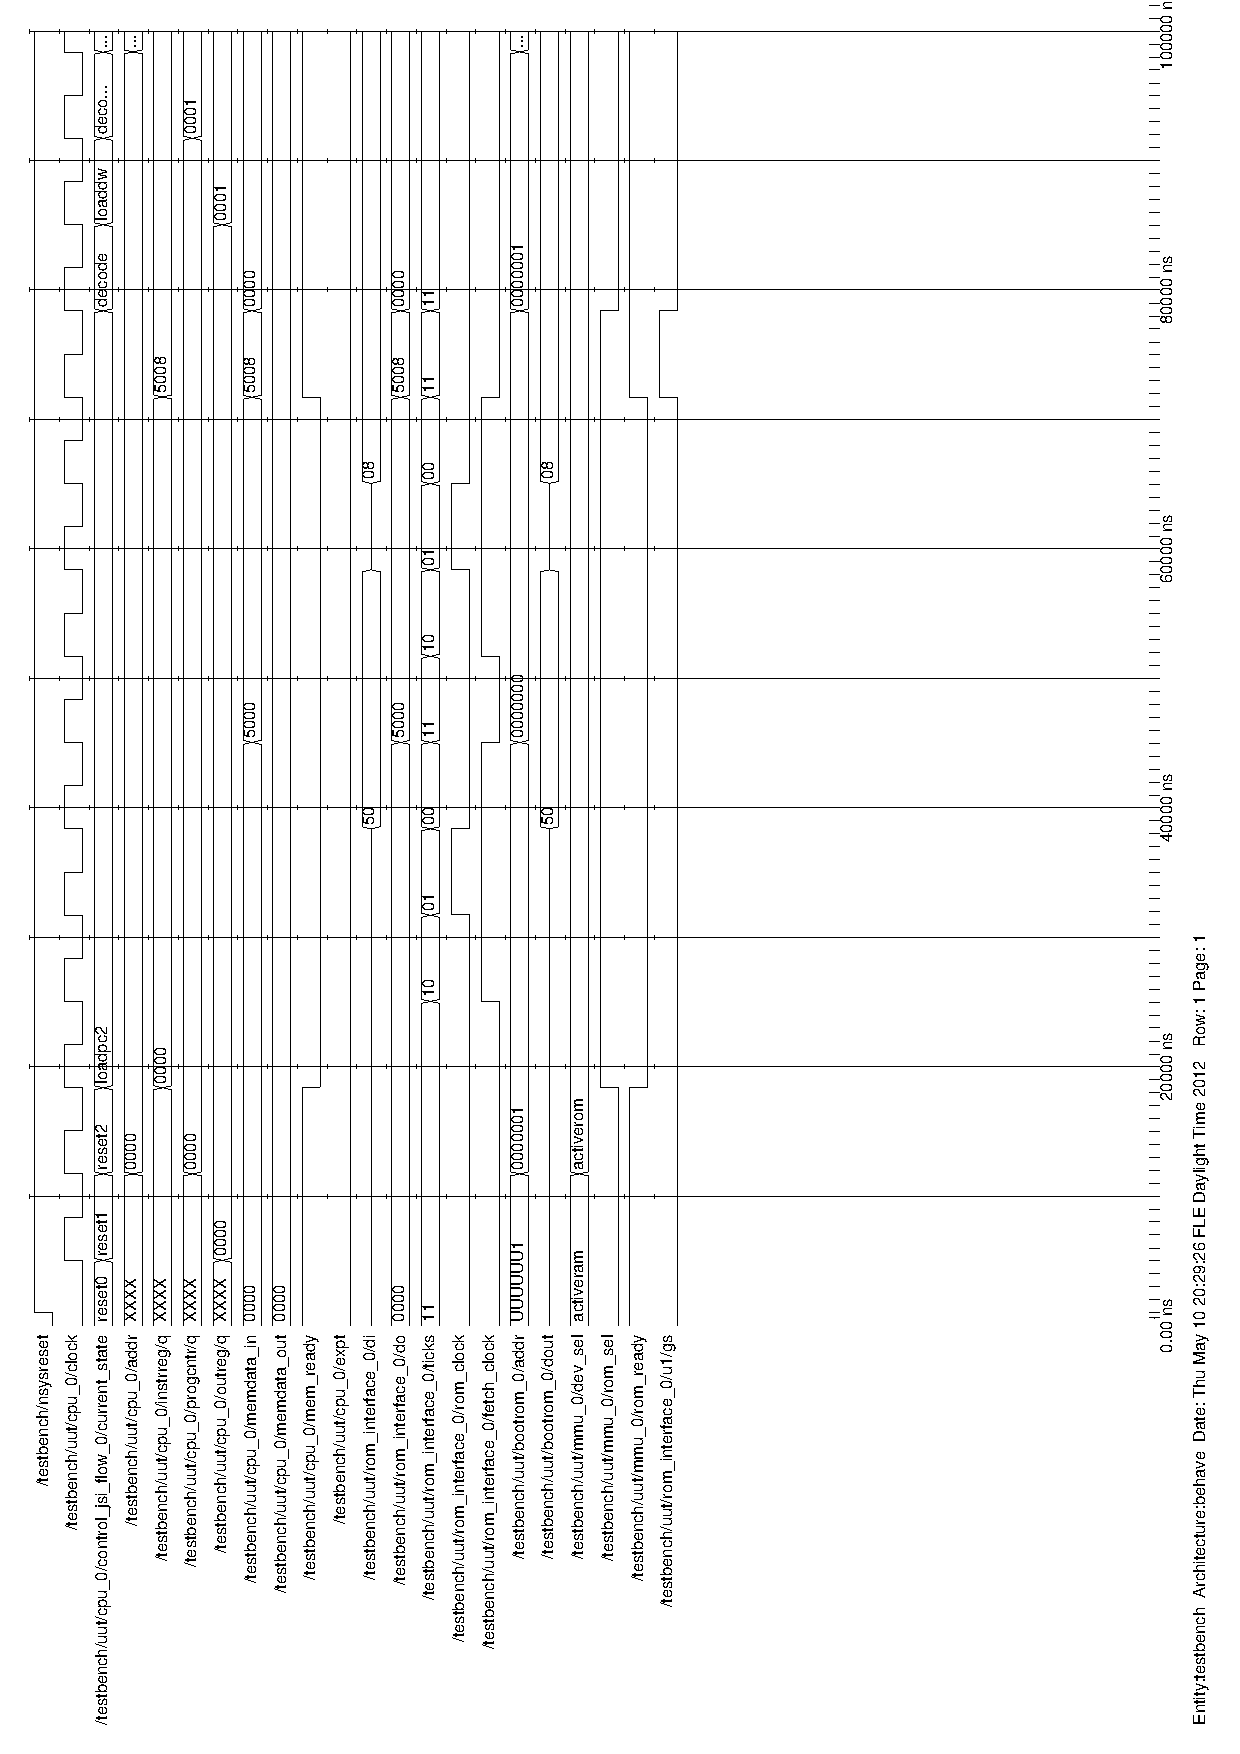
\includegraphics[trim = 0cm 0cm 8.75cm 0cm,clip,angle=-90,width=\linewidth]{sim1_init}\\
	\caption{Mikrokontroliera inicializācijas laika diagramma.}
	\label{fig:sim-boot}
\end{sidewaysfigure}

\begin{sidewaysfigure}
	\centering
	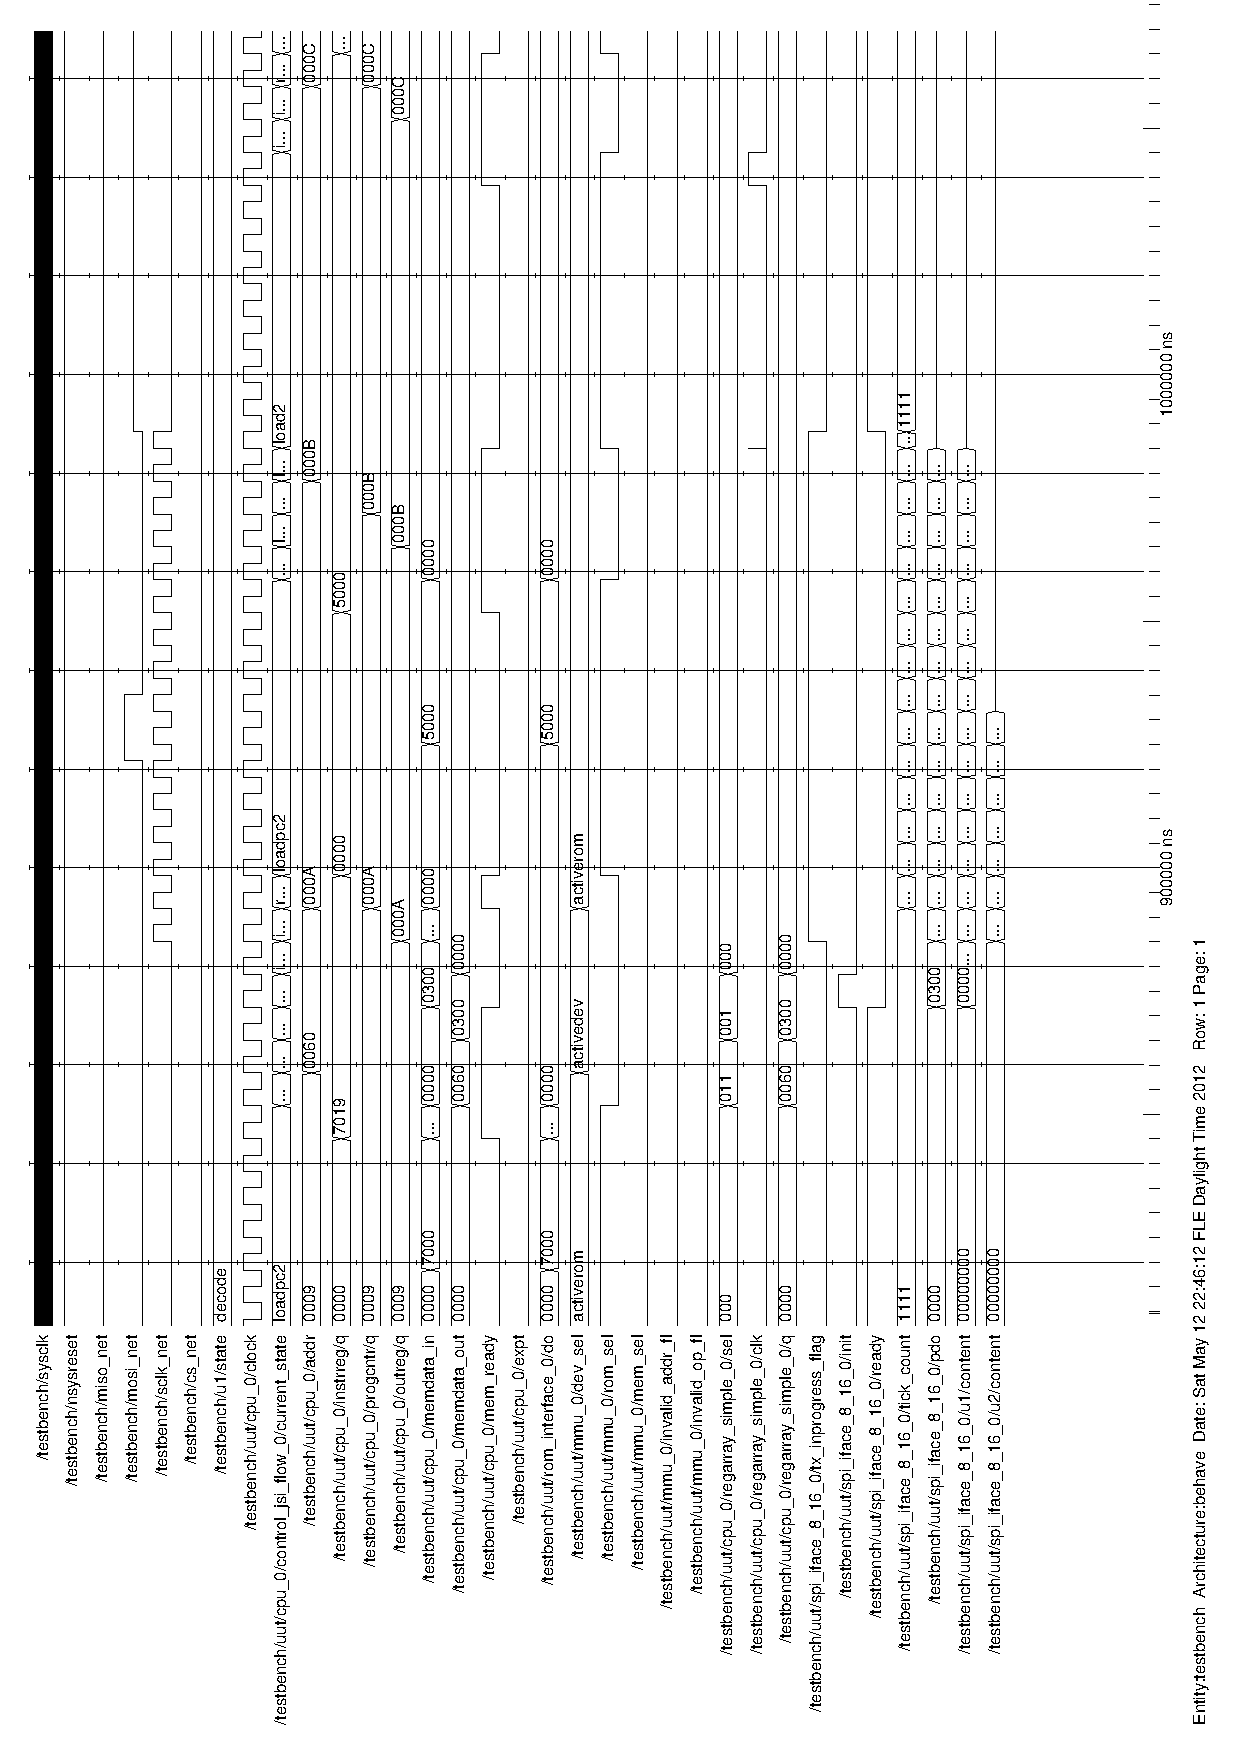
\includegraphics[trim = 0.5cm 0cm 3.25cm 0cm,clip,angle=-90,width=\linewidth]{sim3_tx}\\
	\caption{SPI \termEn{Flash} nolases komandas nosūtīšanas laika diagramma.}
	\label{fig:sim-spi-tx}
\end{sidewaysfigure}

\begin{sidewaysfigure}
	\centering
	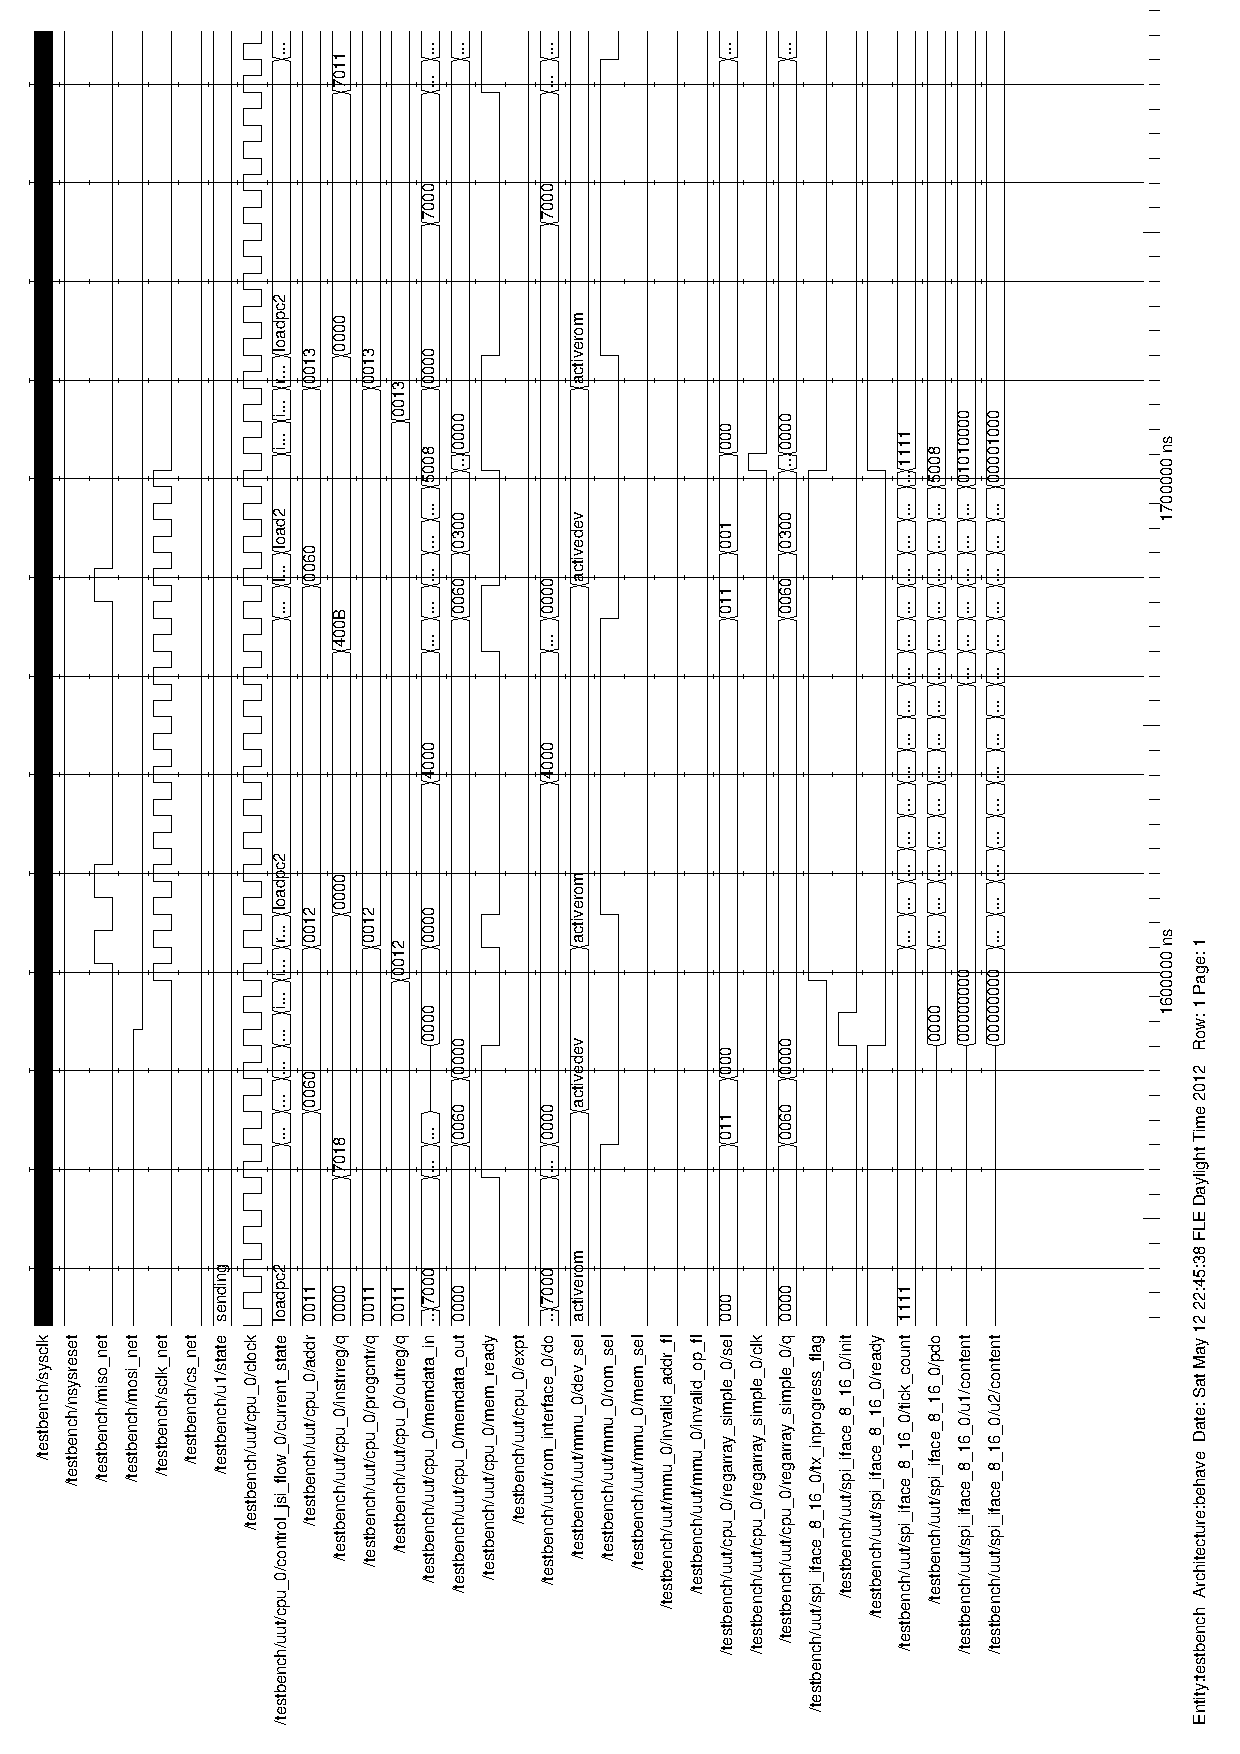
\includegraphics[trim = 0.5cm 0cm 3.25cm 0cm,clip,angle=-90,width=\linewidth]{sim3_rx}\\
	\caption{SPI \termEn{Flash} datu nolases cikla laika diagramma.}
	\label{fig:sim-spi-rx}
\end{sidewaysfigure}
